\documentclass{beamer}

\usepackage{helvet}
\usepackage{hyperref, graphicx}
\usepackage{amsthm}
\usepackage{etoolbox}
\usepackage{wrapfig}
\usepackage{tikz}
\usepackage{ulem}

\usetheme{default}
\setbeamertemplate{navigation symbols}{}
\AtBeginSection[ ]
{
\begin{frame}{Outline}
    \tableofcontents[currentsection]
\end{frame}
}

% Default fixed font does not support bold face
\DeclareFixedFont{\ttb}{T1}{txtt}{bx}{n}{11} % for bold
\DeclareFixedFont{\ttm}{T1}{txtt}{m}{n}{12}  % for normal - use in headings

% Custom colors
\usepackage{color}
\definecolor{TUGray}{RGB}{101,101,137}
\definecolor{TUBlack}{RGB}{30,0,0}
\definecolor{mygreen}{RGB}{45,111,63}
\definecolor{keywords}{RGB}{205,114,0}
\definecolor{comments}{RGB}{181,51,139}
\definecolor{strings}{RGB}{58,144,81}
\definecolor{numeric}{RGB}{66,110,176}
\definecolor{linos}{rgb}{0.4,0.4,0.4}
\definecolor{links}{rgb}{0,0.4,0.75}

\definecolor{bggray}{RGB}{232, 233, 235}

\usecolortheme[named=mygreen]{structure}
\setbeamercolor{normal text}{fg=TUBlack}\usebeamercolor*{normal text}

\setbeamercolor{codecol}{fg=TUGray!25!black,bg=bggray}

\hypersetup{colorlinks, linkcolor=links, urlcolor=links}

\usepackage[T1]{fontenc}
\usepackage[sfdefault,scaled=.85]{FiraSans}
\usepackage{newtxsf}

\usepackage{listings}

\newtoggle{InString}{}% Keep track of if we are within a string
\togglefalse{InString}% Assume not initally in string

\newcommand\digitstyle{\color{numeric}}
\makeatletter
\newcommand{\ProcessDigit}[1]
{%
  \ifnum\lst@mode=\lst@Pmode\relax%
   {\digitstyle #1}%
  \else
    #1%
  \fi
}
\makeatother

\lstset{literate=%
    {0}{{{\ProcessDigit{0}}}}1
    {1}{{{\ProcessDigit{1}}}}1
    {2}{{{\ProcessDigit{2}}}}1
    {3}{{{\ProcessDigit{3}}}}1
    {4}{{{\ProcessDigit{4}}}}1
    {5}{{{\ProcessDigit{5}}}}1
    {6}{{{\ProcessDigit{6}}}}1
    {7}{{{\ProcessDigit{7}}}}1
    {8}{{{\ProcessDigit{8}}}}1
    {9}{{{\ProcessDigit{9}}}}1
	{<=}{{\(\leq\)}}1
	{>=}{{\(\geq\)}}1,
	% morestring=[b]",
    % morestring=[b]',
    % morecomment=[l]{//},
}

\lstdefinelanguage{Pseudo}{
    morekeywords={return, while, if, for, input},
    morecomment=[l]{\#},
}

% Pseudocode style
\newcommand\pseudostyle{\lstset{
language=Pseudo,
basicstyle=\fontfamily{ccr}\scriptsize,
commentstyle=\it\scriptsize\color{linos},
keywordstyle=\it\bfseries\scriptsize,
mathescape=true,
literate=
    {=}{$\leftarrow{}$}{1}
    {==}{$={}$}{1}
    {<=}{{\(\leq\)}}1
	{>=}{{\(\geq\)}}1,
xleftmargin=18pt,
xrightmargin=4pt,
aboveskip=12pt,
belowskip=0pt,
frame=tB,
keepspaces=true
}}

% Python style for highlighting
\newcommand\pythonstyle{\lstset{
language=Python,
basicstyle=\ttfamily\tiny,
numbers=left,
numberstyle=\tiny\color{linos},
morekeywords={self, np},              % Add keywords here
keywordstyle=\tiny\color{keywords},
commentstyle=\it\tiny\color{comments},    % Custom highlighting style
stringstyle=\tiny\color{strings},
xleftmargin=18pt,
xrightmargin=4pt,
aboveskip=0pt,
belowskip=0pt,
escapeinside={(*@}{@*)},
frame=l,                         % Any extra options here
showstringspaces=false,
keepspaces=true
}}

% Pseudocode environment
\lstnewenvironment{pseudo}[1][]
{
    \pseudostyle
    \lstset{
        #1
    }
}
{}

% Python environment 
\lstnewenvironment{python}[1][]
{
	\pythonstyle
	\lstset{
	#1
	}
}
{}

% wrap the Python environment
\newenvironment{codeblock}
    {\hfill\begin{beamerboxesrounded}[lower=codecol, width=0.8\textwidth]
    \medskip

    }
    { 
    \end{beamerboxesrounded}\hfill
    }

\theoremstyle{example}
\newtheorem{question}{Question}

\newcommand{\ct}[1]{\lstinline[language=Python]!#1!}
\newcommand{\ttt}[1]{{\small\texttt{#1}}}
\newcommand{\lsitem}[2]{\ttt{{#1}[}\ct{#2}\ttt{]}}

\author{Chris Cornwell}
\date{Mar 27, 2025}
\title{Gradient descent on Logistic model}

\begin{document}

\begin{frame}
\titlepage
\end{frame}

\section {Gradient Descent in Logistic model}

%%%%
\begin{frame}
\frametitle{Setup}
    As usual, sample data $\mathcal S$; write $({\bf x}_i, y_i)$ for point in $\mathcal S$, with $y_i\in\{1, -1\}$. \newline 
    Parameter space: $\Omega = \mathbb R^{d+1} = \{({\bf w},b)\ |\ {\bf w}\in\mathbb R^d, b\in\mathbb R\}$. For each $\omega \in \Omega$, we have a function $f_{\omega}:\mathbb R^d\to(0,1)$ defined as 
            \[f_{\omega}({\bf x}) = \sigma({\bf w}\cdot{\bf x} + b),\]
    where $\sigma$ is the logistic function. (So, our function output is our probability that the correct label for ${\bf x}$ is $+1$.)
\pause
What do we use for the empirical loss function? When the ``correct'' $y$ is $+1$ (and ${\bf x}$ is far from the hyperplane), we are in a good situation if is $f_{\omega}({\bf x})$ very close to $1$. Alternatively, if the correct $y$ is $-1$, then we would like $f_{\omega}({\bf x})$ to be close to $0$.\newline 
It will help us to alter the numerical values of our labels: for $i$ with $y_i=1$, define $\tilde y_i = 1$; for $i$ with $y_i=-1$, define $\tilde y_i = 0$.\footnote{Functionally, this can be achieved by the definition $\tilde y_i = (y_i+1)/2$.}

\pause 
For these reasons (as well as the rationale for using the logistic function), we use the \textbf{log-loss} function (a.k.a. \textbf{binary cross-entropy}). It is defined by 
    \[\mathcal L_{\mathcal S}(\omega) = \frac{1}{n}\sum_{i=1}^n -\tilde y_i\log(f_{\omega}({\bf x}_i)) - (1-\tilde y_i)\log(1 - f_{\omega}({\bf x}_i)) .\]
\end{frame}

%%%%
\begin{frame}
\frametitle{Gradient descent with logistic regression}
First, compute the gradient of the log-loss function. Pick some $1\le i\le n$, and write the coordinates of the vector ${\bf x}_i\in\mathbb R^d$ as $(x_{i,1},x_{i,2},\ldots,x_{i,d})$. The term in the log-loss from ${\bf x}_i$ is 
        \[-\tilde y_i\log(f_{\omega}({\bf x}_i)) - (1-\tilde y_i)\log(1 - f_{\omega}({\bf x}_i)).\]
If $\tilde y_i = 1$ then this is simply $-\log(f_{\omega}({\bf x}_i))$. Recall that $\sigma(z)$ has a derivative satisfying $\frac{d\sigma}{dz} = \sigma(z)\ast(1 - \sigma(z))$. Using this and the fact that $\frac{d}{dw_j}\left({\bf w}\cdot{\bf x}_i + b\right) = x_{i,j}$, we get 
        \[\frac{d}{dw_j}\left( -\log(f_{\omega}({\bf x}_i)) \right) = - \frac{x_{i,j}\ast f_{\omega}({\bf x}_i)\ast(1 - f_{\omega}({\bf x}_i))}{f_{\omega}({\bf x}_i)} = -x_{i,j}\ast(1-f_{\omega}({\bf x}_i)).\]
The partial with respect to $b$ is simply $-(1-f_{\omega}({\bf x}_i))$.

\end{frame}

%%%%
\begin{frame}
    \frametitle{Gradient descent with logistic regression}
    On the other hand, if $\tilde y_i = 0$ then the term in the log-loss function from ${\bf x}_i$ is $-\log(1-f_{\omega}({\bf x}_i))$. Consequently, we compute 
        \[\frac{d}{dw_j}\left( -\log(1-f_{\omega}({\bf x}_i)) \right) = \frac{x_{i,j}\ast f_{\omega}({\bf x}_i)\ast(1 - f_{\omega}({\bf x}_i))}{1-f_{\omega}({\bf x}_i)} = x_{i,j}\ast f_{\omega}({\bf x}_i),\]
and the partial with respect to $b$ is $f_{\omega}({\bf x}_i)$.

Hence, we have, for each $1\le j\le d$,
    \[\frac{d}{dw_j}\mathcal L_{\mathcal S} = \frac1n\sum_{i=1}^n -\tilde y_ix_{i,j}\ast(1-f_{\omega}({\bf x}_i)) + (1-\tilde y_i)x_{i,j}f_{\omega}({\bf x}_i),\]
and 
    \[\frac{d}{db}\mathcal L_{\mathcal S} = \frac1n\sum_{i=1}^n -\tilde y_i\ast(1-f_{\omega}({\bf x}_i)) + (1-\tilde y_i)f_{\omega}({\bf x}_i).\]
\end{frame}

%%%%
\begin{frame}
    \frametitle{Similarity to Perceptron algorithm updates}
    Consider the \textbf{per-example loss}: given one ``example'' $({\bf x}_i, y_i) \in\mathcal S$, have the term $-\tilde y_i\log(f_{\omega}({\bf x}_i)) - (1 - \tilde y_i)\log(1 - f_{\omega}({\bf x}))$.

    Its partial w.r.t.\ $w_j$ is 
        \[-\tilde y_ix_{i,j}\ast(1-f_{\omega}({\bf x}_i)) + (1-\tilde y_i)x_{i,j}f_{\omega}({\bf x}_i).\]
    If $\tilde y_i=1$, but $f_{\omega}({\bf x}_i)$ is close to 0, then this is \textit{almost} $-y_i x_{i,j}$. Were we to do an update with $\eta=1$ then we would have $w_j^{(t)} \approx w_j^{(t-1)} + y_i x_{i,j}$. This is almost the Perceptron update (in the $j^{th}$ coordinate).

    Likewise, if $\tilde y_i=0$, but $f_{\omega}({\bf x}_i)$ is close to $1$, then the partial is approximately $x_{i,j}$; so, using $\eta=1$, we would get $w_j^{(t)} \approx w_j^{(t-1)} - x_{i,j} = w_j^{(t-1)} + y_ix_{i,j}$. Again, this is almost the Perceptron algorithm update.
\end{frame}

%%%%
\begin{frame}
    \frametitle{Example with Logistic model}
    Given $\pm1$-labeled sample data $\mathcal S= \{({\bf x}_i, y_i)\}_{i=1}^n$, we found an expression for each partial derivative of $\mathcal L_{\mathcal S}$. In fact, if we call $w_{d+1} = b$ and $x_{i,d+1} = 1$ for every $1\le i\le n$, then 
        {\small 
        \[\frac{d}{dw_{j}}\mathcal L_{\mathcal S} = \frac1n\sum_{i=1}^n-\tilde y_ix_{i,j}(1-f_{\omega}({\bf x}_i)) + (1-\tilde y_i)x_{i,j}f_{\omega}({\bf x}_i)\]
        }
    for every $1\le j\le d+1$.

    \textbf{Example:} consider simulated sample data below, drawn uniformly from subset of $[-1,1]^2$ that is at least a fixed distance from $H = \{(x_1,x_2)\in\mathbb R^2\ |\ 2x_1 - \frac23x_2 - \frac15=0\}$. Positively labeled points are in blue. 
    \vspace*{11pt}

    \centering
    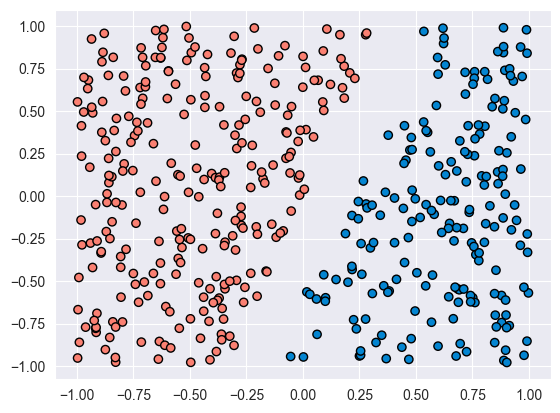
\includegraphics[height=0.3\textheight]{../../Images/simulated-logregression-data.png}
\end{frame}

%%%%
\begin{frame}
    \frametitle{Example with Logistic model}
    Given $\pm1$-labeled sample data $\mathcal S= \{({\bf x}_i, y_i)\}_{i=1}^n$, we found an expression for each partial derivative of $\mathcal L_{\mathcal S}$. In fact, if we call $w_{d+1} = b$ and $x_{i,d+1} = 1$ for every $1\le i\le n$, then 
        {\small 
        \[\frac{d}{dw_{j}}\mathcal L_{\mathcal S} = \frac1n\sum_{i=1}^n-\tilde y_ix_{i,j}(1-f_{\omega}({\bf x}_i)) + (1-\tilde y_i)x_{i,j}f_{\omega}({\bf x}_i)\]
        }
    for every $1\le j\le d+1$.

    \textbf{Example (cont'd):} Batch gradient descent, with learning rate $0.5$, stopping with threshhold $0.0005$, gives (approximately) parameters for: 
        \[\hat{H} = \{(x_1,x_2)\in\mathbb R^2\ |\ 2.01x_1 - 0.63x_2-0.26=0\}.\]
    \centering
    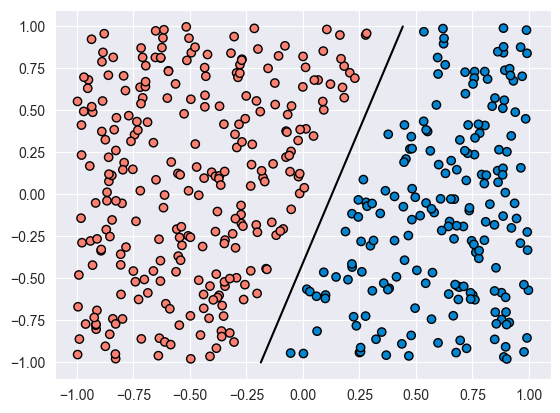
\includegraphics[height=0.3\textheight]{../../Images/Hfit-simulated-logregression-data.png}
\end{frame}

%%%%
\begin{frame}
    \frametitle{Logistic regression on the Iris data}
    Recall the Iris data set: 150 points, 50 from each of three species of Iris flower. Two of the species in the data set, Iris versicolor and Iris virginica, are not linearly separable.

    We can use gradient descent on the logistic model to find a hyperplane that does \textit{well} in classifying the versicolor versus virginica {--} it correctly classifies 97 out of the 100 points.

    For visualization, I first show just the first and fourth coordinates, and the results for logistic model in 2D.

    \centering
    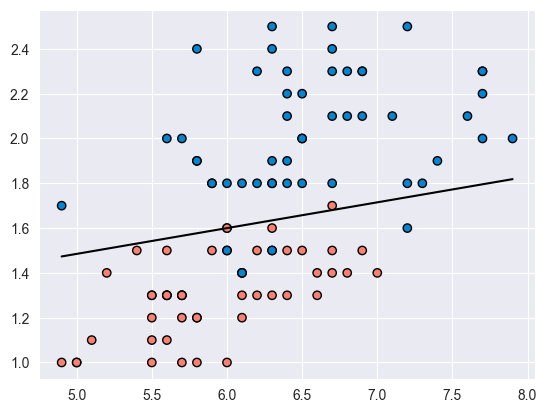
\includegraphics[height=0.35\textheight]{../../Images/HalfSp_2DIrisData.png}
\end{frame}

%%%%
\begin{frame}
    \frametitle{Logistic regression on the Iris data}
    Pictured below are selected lines found during the batch gradient descent. 
    
    As before, yellow-to-purple is progression through the procedure. Consecutive lines that are shown have $200$ updates between them; $\approx 4000$ updates in total.

    The accuracy in this 2D projection is 92\% (the final hyperplane correctly labeled 92 out of 100).\footnote{Recall, the model labels the point with $+1$ when $f_{\omega}({\bf x}) \ge 0.5$.}

    The model on the points in $\mathbb R^4$ took less updates (just under $3000$). It had 97\% accuracy on the data.

    \centering
    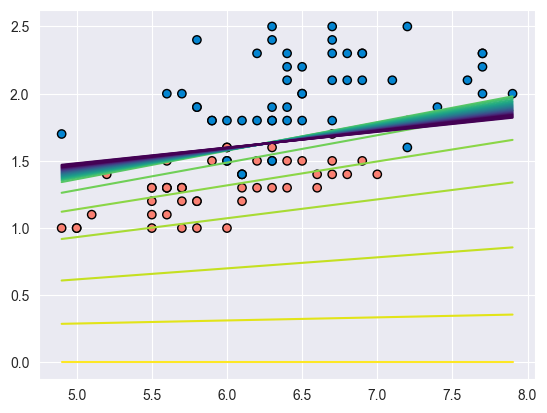
\includegraphics[height=0.35\textheight]{../../Images/GDon2DIrisData.png}
\end{frame}

\end{document}